\section{A Metaprogramming Approach}
\label{Ch5:Sec:Meta}

\begin{comment}
Begin by saying a few words about what metaprogramming is. Then go into subsections. Idea:
1. Establish difficulty of doing computations in \C. Give examples, yes, but also stress that existing automation was unable to unpack the structural nuances of the way \C is defined. Also maybe talk about the whole "is I a numeral" debate, but I think this might be a rabbit-hole...
2. Talk about the algorithm behind norm_numI. Talk about the original version we worked on with Heather and Edison at/after metaprogramming and at Xena.
3. Say something about what Heather's latest modifications look like. Maybe also talk about how the approach can be generalised to quaternion algebras or splitting fields (what's similar and what's different between norm_numI and these things), but don't talk about the maths of either of these. Stress that this is still under development, and that this opens the door to a world of metaprogramming possibilities.
\end{comment}

The formalisation of the solution to the sphere packing problem brought to light a longstanding difficulty faced by the Lean community: a lack of automation for performing computations in $\C$. After a discussion with Heather Macbeth, who is experienced in creating automation for Lean, the author, with Macbeth's guidance and Xie's assistance, embarked on the development of a normalisation-simplification automation procedure for performing computations in $\C$.

% I will condense the stuff below in the shorter (for-submission) version of this thesis. I'll leave it as is over here though... maybe this will come in handy someday...

Lean, like other interactive theorem provers, primarily interacts with its users through \textbf{tactics}. Fundamentally, the proof of a theorem in Lean is given by a \textbf{proof term}, which can be thought of as a concise expression that captures the information of how the hypotheses or inputs of the theorem are transformed into its conclusion by giving exactly the conclusion into which these inputs are transformed. A tactic is a command that, when invoked by a Lean user, performs a step in the construction of the proof term for a theorem.

The most basic tactics can be thought of as being `syntax sugar' rather than invocations of computation or reasoning algorithms. Consider the following code.
% MORE LATEX ERRORS! GAHHHHHHHH
% \begin{lstlisting}[caption=A tactic-mode proof of the associativity of $\land$, label=Ch5:Listing:And_assoc_tactic]
% example (P Q R : Prop) : P ∧ (Q ∧ R) ↔ (P ∧ Q) ∧ R := by
%   constructor
%   · intro h
%     constructor
%     · constructor
%       · exact h.1
%       · exact h.2.1
%     · exact h.2.2
%   · intro h
%     constructor
%     · exact h.1.1
%     · constructor
%       · exact h.1.2
%       · exact h.2
% \end{lstlisting}

This proof demonstrates how the \lstinline|constructor|, \lstinline|intro| and \lstinline|exact| tactics work. These tactics give the Lean compiler the following instructions:
\begin{itemize}
    \item \lstinline|constructor|: ``Prove the goal by proving the two statements it consists of." It works on conjunctions and biconditionals, that is, if the goal is of the form \lstinline|A ∧ B|, then \lstinline|constructor| replaces it with two goals, namely, \lstinline|A| and \lstinline|B|, and if the goal is of the form \lstinline|A ↔ B|, then \lstinline|constructor| replaces it with two goals, namely, \lstinline|A → B| and \lstinline|B → A|.
    
    \item \lstinline|intro|: ``Prove the goal by introducing the assumption term and proving the conclusion term." It works on implications and universal quantifications, that is, if the goal is of the form \lstinline|A → B|, then \lstinline|intro h| introduces an assumption \lstinline|h| of \lstinline|A| and replaces the goal with \lstinline|B|, and if the goal is of the form \lstinline|∀ (x : A), B|, then \lstinline|intro a| introduces term \lstinline|a| of type \lstinline|A| and replaces the goal with \lstinline|B|.

    \item \lstinline|exact|: ``Prove the goal with the following." It works on any goal where the proof of that goal is already known, that is, if the goal is \verb|B| and some proof \lstinline|h| of \lstinline|B| is already known, then \lstinline|exact h| proves the goal with \lstinline|h|.
\end{itemize}

In addition, the terms \lstinline|h.1|, \lstinline|h.2.1|, etc are shorthand for ``the first constituent of \lstinline|h|'', ``the first constituent of (the second constituent of \lstinline|h|)'', etc, where by ``first constituent'' and ``second constituent'', we mean the terms respectively to the left and right of the $\land$ symbol.

What the tactics used in \Cref{Ch5:Listing:And_assoc_tactic} are actually doing is constructing the following \textbf{term-mode proof} of the same result.

\begin{lstlisting}[caption=A term-mode proof of the associativity of $\land$, label=Ch5:Listing:And_assoc_term]
example (P Q R : Prop) : P ∧ (Q ∧ R) ↔ (P ∧ Q) ∧ R :=
  ⟨fun h ↦ ⟨⟨h.1, h.2.1⟩, h.2.2⟩,
   fun h ↦ ⟨h.1.1, ⟨h.1.2, h.2⟩⟩⟩
\end{lstlisting}

% Try and end the discussion here. The point we were trying to make is that tactics generate proof terms. I think that point has been made! The remainder of this section can maybe be a discussion in an appendix. We can say something like "here's some fun facts about theorem proving in Lean" and include this and maybe even some other fun stuff from the book

This proof is significantly shorter than the tactic-mode proof see in \Cref{Ch5:Listing:And_assoc_tactic}. While the code is arguably less readable than the tactic-mode proof, it is not too difficult to dissect:
\begin{itemize}
    \item The \lstinline|constructor| occurrences in \Cref{Ch5:Listing:And_assoc_tactic} correspond to the \textit{anonymous constructors} \lstinline|⟨,⟩| in \Cref{Ch5:Listing:And_assoc_term}.

    \item The \lstinline|intro h| occurrences in \Cref{Ch5:Listing:And_assoc_tactic} correspond to the function definitions \lstinline|fun h ↦| in \Cref{Ch5:Listing:And_assoc_term}.

    \item The \lstinline|exact| occurrences in \Cref{Ch5:Listing:And_assoc_tactic} correspond to the terms inside the anonymous constructors in \Cref{Ch5:Listing:And_assoc_term}.
\end{itemize}

In particular, the proof in \Cref{Ch5:Listing:And_assoc_term} consists solely of functions and constructors. No tactics occur anywhere in the argument (note the absence of the \lstinline|by| keyword, which marks the beginning of a tactic-mode proof).

It turns out that \Cref{Ch5:Listing:And_assoc_term} still contains some syntax sugar. It is possible to use helper lemmas like \verb|Iff.intro| and \verb|And.intro| to avoid using the anonymous constructors, but a proof term completely devoid of the constructor syntax would look like the following.

% Why am I getting LaTeX errors here????????
% \begin{lstlisting}[caption=A proof term for the associativity of $\land$, label=Ch5:Listing:And_assoc_proof_term, escapeinside=``]
% example (P Q R : Prop) : P ∧ (Q ∧ R) ↔ (P ∧ Q) ∧ R := {
%   mp := fun a ↦ {
%     left := {
%       left := And.casesOn a fun left right ↦ And.casesOn right fun _ _ ↦ left
%       right := And.casesOn a fun _ right ↦ And.casesOn right fun left _ ↦ left
%     }
%     right := And.casesOn a fun _ right ↦ And.casesOn right fun _ right ↦ right
%   }
%   mpr := fun a ↦ {
%     left := And.casesOn a fun left _right ↦ And.casesOn left fun left _ ↦ left `\newpage`
%     right := {
%       left := And.casesOn a fun left _ ↦ And.casesOn left fun _ right ↦ right
%       right := And.casesOn a fun left right ↦ And.casesOn left fun _ _ ↦ right
%     }
%   }
% }
% \end{lstlisting}

Proof terms, as we can see from \Cref{Ch5:Listing:And_assoc_proof_term}, are often long and do not clearly communicate the mathematical ideas they represent. Tactics overcome this by constructing proof terms without revealing them to the user. Indeed, there are tactics that serve as more than just syntax sugar: for example, results in intuitionistic propositional logic (such as the associativity of $\land$) can be proved by the tactic \lstinline|itauto|. That is, the following code compiles.


\begin{lstlisting}[caption=A one-line tactic proof for the associativity of $\land$, label=Ch5:Listing:And_assoc_itauto]
example (P Q R : Prop) : P ∧ (Q ∧ R) ↔ (P ∧ Q) ∧ R := by itauto
\end{lstlisting}

Other tactics like \lstinline|tauto| and \lstinline|simp| also work. The proof term generated by such a tactic can be viewed by typing \lstinline|show_term|.\footnote{For the curious reader, \Cref{Ch5:Listing:And_assoc_proof_term} was generated by repeatedly typing \lstinline|show_term by tauto| inside each field.} For a more detailed explanation of how proof terms and tactics work, see \cite[particularly Chapters 3 and 5]{ThmPfInLean}.

\textbf{Metaprogramming} is the science of writing tactics in Lean. While syntax-sugar tactics are incredibly useful (compare the readability of \Cref{Ch5:Listing:And_assoc_tactic,Ch5:Listing:And_assoc_term,Ch5:Listing:And_assoc_proof_term}), automation tactics often go an even longer way in keeping the focus of nontrivial mathematical proofs on precisely their nontrivial aspects. Given how computationally involved the construction of Viazovska's Magic Function is (as seen in \Cref{Ch4:Chapter}), the author, after a discussions with Macbeth, realised that the most efficient approach to formalising some of the computational aspects of Viazovska's argument was to write a tactic. The first version of this tactic, developed as a collaboration between Macbeth, Xie and the author, with inputs from Mehta, was called \lstinline|norm_numI|.

In the forthcoming subsections, we explore the motivation and technique used to develop \lstinline|norm_numI|, and briefly discuss how the tactic maybe further developed and the scope of its applicability expanded.

\subsection{Complex Computations are Complex}

Computations in general are quite challenging to perform in interactive theorem provers. This is because such languages are designed for \textit{proof} rather than \textit{computation}. Indeed, tactics that simplify goals do not do so merely by simplifying expressions: they construct proofs that the simplified expression is, indeed, equal to the original expression. Existing tactics like \lstinline|norm_num|, \lstinline|simp| and \lstinline|field_simp| do not always do this successfully when the expressions in question are in $\C$. \lstinline|simp| and \lstinline|field_simp| are very general tactics that work in a wide variety of settings. They both work by constructing a special set of equality or biconditional lemmas by sifting through the library and performing repeated rewrite operations to transform the goal into a simpler form. \lstinline|field_simp| is specifically designed to simplify expressions in fields, and can handle operations like clearing denominators. However, it does not have access to the particularities of the field in question (such as the fact that $i^2 = -1$ in $\C$). The tactic that we will be most interested in, specifically because it is designed to handle simplifications of \textit{numerals} in \textit{specific} settings, is \lstinline|norm_num|.

\lstinline|norm_num| is a tactic that handles expressions involving numerals. It works best in $\N$, $\Z$ and $\Q$. For example, it handles the following.
% \begin{lstlisting}[caption={\lstinline|norm_num| simplifying expressions in $\N$, $\Z$ and $\Q$}]
% example : (1 : ℕ) + 2 + 3 + 4 = 10 := by norm_num
% example : (-2 : ℚ) * (3 + 8/9) = -70/9 := by norm_num
% example : (-9 : ℤ) + 5 * (6 - 20) = -79 := by norm_num
% \end{lstlisting}
It is worth mentioning, however, that \lstinline|norm_num| often has difficulties in $\R$. This is due to the immense technical detail baked into the very definition of $\R$ in Lean, which allows for the existence of transcendental numbers. In the following example, none of \lstinline|norm_num|, \lstinline|field_simp|, \lstinline|ring| and \lstinline|simp| can prove the result in one line, because they are unable to treat $\pi$ as more than a symbol. Indeed, the entire proof rests on a \mathlib\ result, \lstinline|Real.pi_gt_three|.

\begin{lstlisting}[caption=An expression in $\R$ not handled immediately by simplification tactics, label=Ch5:Listing:pi_sub_one_norm_num_fail]
example : (π - 1) / (π - 1) = 1 := by
  have h₁ : (1 : ℝ) < 3 := by norm_num
  have h₂ : 1 ≠ π := ne_of_lt <| h₁.trans pi_gt_three
  have h₃ : π - 1 ≠ 0 := sub_ne_zero_of_ne h₂.symm
  field_simp [h₃]
\end{lstlisting}

Observe, however, that \lstinline|norm_num| \textit{is} able to prove the inequality $1 < 3$ despite it being an expression in $\R$. The reason is that \lstinline|norm_num| can navigate the canonical inclusions from $\N$, $\Z$ and $\Q$ into $\R$, meaning that it can simplify expressions in $\R$ that come from expressions it can simplify in $\N$, $\Z$ or $\Q$.\footnote{We say \lstinline|norm_num| can handle coercions.} It cannot, however, show that $1 < \pi$, because it does not treat $\pi$ \textit{as a numeral}. In $\C$, \lstinline|norm_num| faces this challenge not only with real transcendental numbers like $\pi$ but also with the imaginary constant $i$. Consider the following example.\footnote{Note that in Lean, the imaginary constant is denoted by an uppercase \lstinline|I| instead of a lowercase $i$. We will adhere to standard mathematical conventions and use a lowercase $i$ when referring to the imaginary constant in informal contexts.}

\begin{lstlisting}[caption={A nontrivial computation in $\C$, done formally}, label=Ch5:Listing:long_tactic_pf_example_complex]
example : (1 + I) * (1 + I * I * I) = 2 := by
  simp only [I_mul_I, neg_mul, one_mul, mul_add, mul_one, mul_neg, add_mul, neg_add_rev, neg_neg]
  ring
\end{lstlisting}

Again, \lstinline|simp|, \lstinline|field_simp|, \lstinline|ring| and \lstinline|norm_num| all fail, because $i$, like $\pi$ in \Cref{Ch5:Listing:pi_sub_one_norm_num_fail}, is not handled as a numeral. Observe, however, that $\parenth{1 + i}\parenth{1 + i \cdot i \cdot i}$ lies in $\Z[i]$. This means that if it is expressed as $a + bi$, with $a$ and $b$ both being (not necessarily simplified) real expressions, then in fact, $a$ and $b$ are both images of expressions in $\Z$. This means that \lstinline|norm_num| would be able to individually handle both $a$ and $b$, resulting in a simplified expression of the form $a' + b'i$, with $a'$ and $b'$ being simplified. This suggests that the key to writing a tactic that can simplify expressions like those in \Cref{Ch5:Listing:long_tactic_pf_example_complex} is to find a way to separate them into their real and imaginary parts, which in turn involves navigating the fact that $i^2 = -1$.

\subsection{Parsing and Normalisation}

The core idea behind \lstinline|norm_num| is that it simplifies expressions by computing normal forms. In its most basic form, \lstinline|norm_num| attempts to prove equalities of by putting the left and right hand sides in unique normal forms that can simply be inspected to check if the two sides are equal. For example, in the natural numbers, simple arithmetic facts are true by \textit{reflexivity}, that is, they are proved by the tactic \lstinline|rfl|, which proves definitional equality. Hence, the right normal form for numerical expressions in $\N$ is to just compute them and express them as a single natural number (ie, as the right number of applications of the successor function to $0$). Then, by inspection, two expressions are equal if and only if their normal forms---that is, their simplifications into single natural numbers---are equal. Inequalities work similarly.

While the working of \lstinline|norm_num| may appear trivial in $\N$, its versatility becomes clearer in \textit{semirings}. Recall that a semiring is an algebraic structure that is a commutative, additive monoid and a multiplicative monoid, with the quintessential example being $\N$. If $A$ is any semiring, there is a natural semiring homomorphism $\uparrow : \N \to A$ given by
\begin{align*}
    \uparrow\!0 &:= 0 \\
    \uparrow\!1 &:= 1 \\
    \uparrow\!2 &:= 1 + 1 \\
    &\ \ \ \vdots
\end{align*}
A \textbf{numeral} in $A$ is then any element of the image of $\uparrow$, and \lstinline|norm_num| puts expressions involving numerals in normal forms by recognising them as numerals, computing the normal form of their pre-images in $\uparrow$, and pushing the image back through $\uparrow$. The nontriviality of \lstinline|norm_num| for numerical expressions in $A$ is then not how it computes normal forms in $\N$ but how it navigates $\uparrow$. For more on how \lstinline|norm_num| works in semirings, follow the tutorial in \cite[\texttt{Metaprogramming/NormNum}]{HeatherMetaprogramming}. We will not discuss it in any more detail here, but will instead discuss the working of \lstinline|norm_numI|---specifically, what the desired normal form is and how it is computed.

Since $\R$ is a subfield of $\C$, the constraints that the standard \lstinline|norm_num| faces in $\R$ are also constraints it can reasonably be expected to face in $\C$. The goal of \lstinline|norm_numI| is not to overcome \textit{these} constraints, but to overcome the \textit{additional} constraints that come from not treating $i$ as a numeral. The target normal form for an expression in $\C$ is therefore given by separating it into its real and imaginary parts, both of which are real expressions, and normalising them as much as possible.

The key to \lstinline|norm_numI| is the \href{https://github.com/thefundamentaltheor3m/Sphere-Packing-Lean/blob/05f51ee8f61972da1b0a5ee360c4c57c1b599cca/SpherePacking/Tactic/NormNumI.lean#L72}{\lstinline|parse| function}. It separates an expression $z \in \C$ into its real and imaginary parts by performing a recursive pattern-match. For example, if the outermost operation is addition---ie, if $z = z_1 + z_2$---then it calls itself on both $z_j$, obtaining real and imaginary parts $a_j, b_j \in \R$ and proofs that $z_j = a_j + b_ji$, and returns the expression $\parenth{a_1 + a_2} + \parenth{b_1 + b_2}i$ as well as a proof that $z = \parenth{a_1 + a_2} + \parenth{b_1 + b_2}i$, which it obtains via a helper lemma \href{https://github.com/thefundamentaltheor3m/Sphere-Packing-Lean/blob/05f51ee8f61972da1b0a5ee360c4c57c1b599cca/SpherePacking/Tactic/NormNumI.lean#L20}{\lstinline|split_add|}. It performs similar recursive actions if $z$ is of the form $z_1 \cdot z_2$, $z_1\inv$, $z_1 / z_2$, $-z_1$, $z_1 - z_2$, $\overline{z_1}$, $z_1^n$ for some $n \in \N$, $i$, or a decimal/natural number. The recursion is guaranteed to terminate, because an expression that is fed into the function cannot contain infinitely many characters.

\begin{boxexample}\label{Ch5:Eg:Parse}
    The expression $z = \parenth{1 + i}\parenth{1 + i \cdot i \cdot i}$ (cf. \Cref{Ch5:Listing:long_tactic_pf_example_complex}) would be parsed in the following manner.
    \begin{enumerate}[noitemsep]
        \item To parse $z$, write $z = z_1 \cdot z_2$, where $z_1 = 1 + i$ and $z_2 = 1 + i \cdot i \cdot i$.
        \item To parse $z_1$, write $z_1 = z_{11} + z_{12}$ where $z_{11} = 1$ and $z_{12} = i$.
        \item $z_{11}$ is parsed as $1 + 0i$.
        \item $z_{12}$ is parsed as $0 + 1i$.
        \item By \lstinline|split_add|, $z_1 = z_{11} + z_{12}$ is parsed as
              \begin{align*}
                  \parenth{1 + 0} + \parenth{0 + 1}i
              \end{align*}
        \item To parse $z_2$, write $z_2 = z_{21} + z_{22}$, where $z_{21} = 1$ and $z_{22} = i \cdot i \cdot i$.
        \item $z_{21}$ is parsed as $1 + 0i$.
        \item To parse $z_{22}$, write $z_{22} = z_{221} \cdot z_{222}$, where $z_{221} = i \cdot i$ and $z_{222} = i$.
        \item To parse $z_{221}$, write $z_{221} = z_{2211} \cdot z_{2212}$, where $z_{2211} = i$ and $z_{2212} = i$.
        \item $z_{2211}$ is parsed as $0 + 1i$.
        \item $z_{2212}$ is parsed as $0 + 1i$.
        \item By \lstinline|split_mul|, $z_{221} = z_{2211} \cdot z_{2212}$ is parsed as
              \begin{align*}
                  \parenth{0 \cdot 0 - 1 \cdot 1} + \parenth{0 \cdot 1 + 0 \cdot 1}i
              \end{align*}
        \item $z_{222}$ is parsed as $0 + 1i$.
        \item By \lstinline|split_mul|, $z_{22} = z_{221} \cdot z_{222}$ is parsed as
              \begin{align*}
                  \parenth{
                    \parenth{0 \cdot 0 - 1 \cdot 1}
                        \cdot
                    0
                    -
                    \parenth{0 \cdot 1 + 1 \cdot 0}
                        \cdot
                    1
                  } + \parenth{
                    \parenth{0 \cdot 0 - 1 \cdot 1}
                        \cdot
                    1
                    +
                    0
                        \cdot
                    \parenth{0 \cdot 1 + 1 \cdot 0}
                  }i
              \end{align*}
        \item By \lstinline|split_add|, $z_2 = z_{21} + z_{22}$ is parsed as
              \begin{align*}
                  &\parenth{1 + \parenth{
                    \parenth{0 \cdot 0 - 1 \cdot 1}
                        \cdot
                    0
                    -
                    \parenth{0 \cdot 1 + 1 \cdot 0}
                        \cdot
                    1
                  }} \\
                  + &\parenth{0 + \parenth{
                    \parenth{0 \cdot 0 - 1 \cdot 1}
                        \cdot
                    1
                    +
                    0
                        \cdot
                    \parenth{0 \cdot 1 + 1 \cdot 0}
                  }}i
              \end{align*}
        \item By \lstinline|split_mul|, $z = z_1 + z_2$ is parsed as
              \hspace{-2em}
              \begin{align*}
                  &\Big(
                    \parenth{1 + 0}
                        \cdot
                    \parenth{1 + \parenth{
                        \parenth{0 \cdot 0 - 1 \cdot 1}
                            \cdot
                        0
                        -
                        \parenth{0 \cdot 1 + 1 \cdot 0}
                            \cdot
                        1
                    }} \\
                    & -
                    \parenth{0 + 1}
                        \cdot
                    \parenth{0 + \parenth{
                        \parenth{0 \cdot 0 - 1 \cdot 1}
                            \cdot
                        1
                        +
                        0
                            \cdot
                        \parenth{0 \cdot 1 + 1 \cdot 0}
                    }}
                  \Big) \\
                  + &\Big(
                    \parenth{1 + 0}
                        \cdot
                    \parenth{0 + \parenth{
                        \parenth{0 \cdot 0 - 1 \cdot 1}
                            \cdot
                        1
                        +
                        0
                            \cdot
                        \parenth{0 \cdot 1 + 1 \cdot 0}
                    }} \\
                    & +
                    \parenth{1 + \parenth{
                        \parenth{0 \cdot 0 - 1 \cdot 1}
                            \cdot
                        0
                        -
                        \parenth{0 \cdot 1 + 1 \cdot 0}
                            \cdot
                        1
                    }}
                        \cdot
                    \parenth{0 + 1}
                  \Big)i
              \end{align*}
    \end{enumerate}
\end{boxexample}

\begin{wrapfigure}{r}{0.4\linewidth}
    \centering
    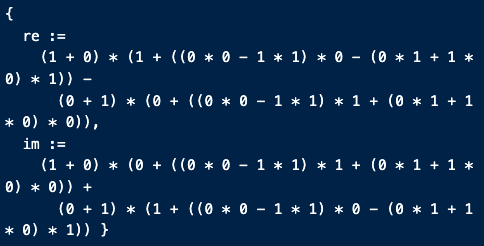
\includegraphics[width=0.95\linewidth]{Chapters/5_Lean/Images/norm_numI_parse_output.png}
    \caption{The Lean output of the steps shown in \Cref{Ch5:Eg:Parse}.}
    \label{Ch5:Fig:Parse_Example}
\end{wrapfigure}

Note that in Lean, the result of parsing does not appear as an expression of the form $a + bi$, but rather, as a \lstinline|structure| with fields \lstinline|re| and \lstinline|im| for the real and imaginary parts. However, the underlying idea is no different from what we have described.

Clearly, despite being mathematically valid, the result of parsing can be long and uninformative, making it an unsuitable choice of normal form for our purposes. However, by separating complex expressions into their real and imaginary parts, \lstinline|parse| perfectly sets up a very simple normalisation procedure that will put our expression in an appropriate normal form. Since we know of such a procedure for real expressions---namely, \lstinline|norm_num|---and since \lstinline|parse| expresses any complex expression as a combination of two real expressions, the normalisation procedure simply makes calls to \lstinline|norm_num| to express each of them in a \textit{real} normal form. The result is a complex number in a normal form $a + bi$ (or, in Lean notation, \lstinline|{re := a, im := b}|) with $a$ and $b$ both simplified to the greatest extent possible (as expressions in $\R$) by applying \lstinline|norm_num|.

Note that \lstinline|norm_numI| is currently implemented as a \lstinline|conv| tactic rather than a full tactic, meaning that it is only capable of modifying expressions (and providing a proof that the modification is valid). It is not currently capable of proving goals, which are necessarily logical statements, such as equalities. This means that it needs to be used as follows.

% Why is there an error in the following listing?
% Uncomment before submitting. Keep commented till then so easier to keep track of errors.
% \begin{lstlisting}[caption={Using \lstinline|norm_numI| as a \lstinline|conv| tactic}, label=Ch5:Listing:norm_numI_as_conv]
% example : (1 + I) * (1 + I * I * I) = 2 := by
%   conv_lhs => norm_numI
%   conv_rhs => norm_numI
% \end{lstlisting}

Unpacking the code,
\begin{itemize}
    \item \lstinline|conv_lhs => norm_numI| applies the parsing-normalisation procedure outlined above to convert the expression \lstinline|(1 + I) * (1 + I * I * I)| on the left-hand side to \lstinline|{re := 2, im := 0}|.
    \item \lstinline|conv_rhs => norm_numI| applies the parsing-normalisation procedure outlined above to convert the expression \lstinline|2| on the right-hand side to \lstinline|{re := 2, im := 0}|.
\end{itemize} 
Since the two sides are then exactly the same, the goal is proved. Note that both lines are necessary: $2$ on its own has not been separated into real and imaginary parts. The imaginary part needs to be explicitly shown to be $0$, which the \lstinline|parse| function does.

After Macbeth, Xie and the author's initial success with this \lstinline|conv| tactic, Macbeth proceeded to create an \textit{extension} of the existing \lstinline|norm_num| tactic that uses the parsing technique outlined above to handle complex expressions. This tactic is still being developed, but is being tested on active code from the project with immensely promising results.

\subsection{Scope for Further Development}

The benefits of having such a tactic cannot be overstated. There are numerous instances across the project where the collaborators have had to repeatedly prove computational facts in $\C$, such as $1 + i \neq 0$, or clear complex denominators to separate expressions into their real and imaginary parts. It is precisely this that motivated the development of \lstinline|norm_numI|, and indeed, \lstinline|norm_numI| is proving to be a viable solution.

% Give an explicit example here from the repo

The applicability of \lstinline|norm_numI|---or, at the very least, of the underlying idea, that the right normal form for expressions in $\C$ is to separate them into real and imaginary parts and express those in a normal form---extends well beyond expressions in $\C$. A key motivation for Xie, one of the co-creators of \lstinline|norm_numI| and an ardent algebraist, was to create a similar tactic that would normalise and simplify expressions in quaternion algebras. A discussion at a London Learning Lean event hosted at the London Institute of Mathematical Sciences in March 2025 sparked speculation among well-regarded members of the Lean Community that similar ideas might be applicable in other field extensions (with $\C$ regarded as $\quotient{\R[X]}{\parenth{X^2 + 1}}$ and $i$ as the image of $X$ via the quotient map). The idea would be that the separation into components corresponds to taking advantage of some linear independence criterion, with algebraic dependences not handled by the simplification step being captured by the helper lemmas in the normalisation step.

There are numerous technical difficulties with implementing such a tactic that can work in other contexts, chief amongst them the fact that there would need to be a single modification to the tactic capable of handling very differently behaved algebraic structures (for instance, it would need to work the same way in quadratic, cubic, quartic and higher degree field extensions). It would hence need to have some awareness of the behaviours of each field in which it is applied, which is technically challenging. Nevertheless, the development of \lstinline|norm_numI| and the subsequent \lstinline|norm_num| modification marks a significant, and long overdue, step in the right direction, so that fewer nontrivial proofs are needed to prove trivial facts.